\documentclass[conference]{IEEEtran}
\IEEEoverridecommandlockouts
% The preceding line is only needed to identify funding in the first footnote. If that is unneeded, please comment it out.
\usepackage{cite}
\usepackage{amsmath,amssymb,amsfonts}
\usepackage{algorithmic}
\usepackage{graphicx}
\usepackage{textcomp}
\usepackage{hyperref}
\usepackage{xcolor}
\usepackage[section]{placeins}
\def\BibTeX{{\rm B\kern-.05em{\sc i\kern-.025em b}\kern-.08em
    T\kern-.1667em\lower.7ex\hbox{E}\kern-.125emX}}
\begin{document}

\title{Experiment 4\\
{  Game Playing Agent - Minimax - Alpha-Beta Pruning
}
}

\author{\IEEEauthorblockN{Harsh Mehta}
\IEEEauthorblockA{\textit{202051117} \\
}
\and
\IEEEauthorblockN{Mohd. Amber Rizvi}
\IEEEauthorblockA{\textit{202051121} \\
}
\and
\IEEEauthorblockN{Om Nalinde}
\IEEEauthorblockA{\textit{202051125} \\
}
\and
\IEEEauthorblockN{Akhilesh Manda}
\IEEEauthorblockA{\textit{202051015} \\
}
}

\maketitle

\section{Abstract}
The objective of this study is to utilize the Minimax algorithm, along with improvisation techniques using alpha beta pruning, to analyze and optimize the game of noughts and crosses. Additionally, this research aims to demonstrate that, regardless of the moves made by player 1, player 2 will always win in the game of Nim by employing the minimax value backup argument on the game tree.


\section{Introduction}
To begin our discourse, we introduce the following topics:
\begin{itemize}
    \item Playing Agent: Referring to a machine or human entity that is capable of performing actions, or a program specifically designed for playing strategic games such as Chess or Go.
    \item Minimax: A recursive algorithm that traverses the entire tree structure and calculates the minimax values by returning values through the tree during the recursive unwinding process.
    \item Alpha Beta Pruning: A technique that enhances the Minimax algorithm by pruning or eliminating the unnecessary subtrees to save computation time, and thereby improving the overall efficiency of the algorithm.
\end{itemize}

\section{Tic-Tac-Toe}
The game is played between two agents, where each agent alternates in marking the symbols X or O on a 3 × 3 grid. Assuming that both agents are playing optimally, the game will ultimately result in a draw.
\subsection{Define the game}
\[Game({S_0}) = \begin{bmatrix}
\__ & \__ &\__\\
\__ & \__ &\__\\
\__ & \__ &\__
\end{bmatrix}\]
\\\
On observing we see that given any player starts the game, The first player will have 9 choices, the next player has 8 and so on, therefore the grid can be filled in $ways = 9*8*7*6*5*4*3*2*1$ = $9!$. This is considering that each position is different irrespective of the rotations possible on the board.

The total possible states = $3^9$ which considers all possible distributions of X,O,blank in the grid (invalid moves also). If we take into account the number of nodes that are traversed, while considering all the distinct states and sequences, including instances where the end state is the same but the order of moves differs, then it is estimated that the game tree will contain approximately 1 million nodes (or 10 Lakh nodes).

\begin {center}
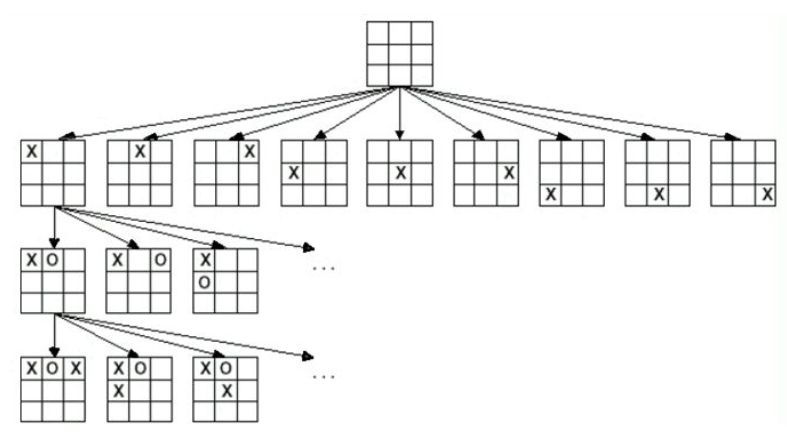
\includegraphics[width=0.49\textwidth]{minmax.png}
\caption{Game Tree Sketch} % Caption change
\label{fig:ecg}
\end {center}

\section{The Game of Nim}
The game of Nim is a competitive activity that involves two players, with each participant taking turns in removing objects from designated piles. The ultimate goal of the game is to strategically force one's opponent into a position where they are compelled to take the final object, rendering them unable to make any additional moves and ultimately resulting in their defeat. In this study, we will examine a specific stack that is represented in Figure 1, under the assumption that both players will adopt optimal strategies. Through our analysis, it has been determined that the player who moves first will always suffer a loss, while the second player will consistently emerge victorious.

\begin{center}
    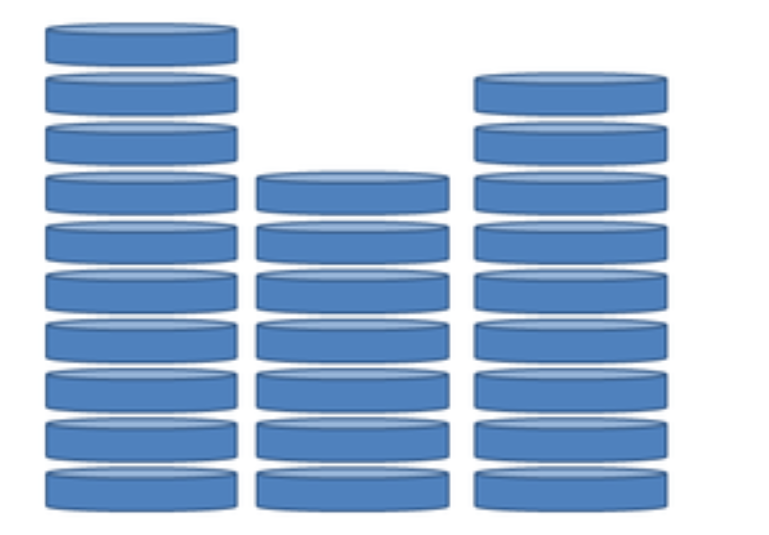
\includegraphics[scale=0.58]{Nim game.png}\\
    \caption{ Fig.2.Nim Game Initial Configuration}
\end{center}

In the game of Nim, victory is determined by two key factors: the player who initiates the game, and the initial configuration of the game. Specifically, the configuration of the game is comprised of three piles, with the first pile containing 10 discs (8+0+2+0), the second pile containing 7 discs, and the final pile comprising 9 discs. To achieve victory, Player 2 must always ensure that they leave Player 1 with a Nim sum of zero. However, the current configuration of the piles shows that there are four extra discs in the second pile, resulting in a non-zero Nim sum. It is important to note that each pile's discs represent the sum of powers of two, which further contributes to the non-zero initial Nim sum.

In the scenario where Player 1 selects a random disc from any pile, several possibilities arise. If Player 1 chooses one to three discs from pile 2, then Player 2 is compelled to select four discs from the remaining pair, as designated by the pair [(1,1),(2,2),(8,8)]. However, if Player 1 selects any other options, then Player 2 must remove four discs from the second pile to ensure victory. This scenario is designated as Case 1.

Case 2: The next step involves both players confirming whether the sum of the Nim piles is balanced, meaning the sum of the pile's values is zero. The game continues as long as there are objects in any pile, and on each turn, player 1 makes the Nim sum non-zero, and player 2 balances it back to zero until there are no objects left. At this point, player 2, who made the last move, wins the game.

Case 3: To ensure that player 2 wins, player 1 must select the last object. Assuming that piles 1 and 3 each have the final set of four objects, which is possible because groups of 2, 4, or 8 can be divided to balance and make the Nim sum zero, player 1 will make the next moves.

If Alpha Beta Pruning could be done in the most effective way
then the Time Complexity for the same will be $O(b^{m/2})$.
\[T(m) = T(m − 1) + (b − 1)T(m − 2)\]
\[T(m) = O(b^{m/2})\]
This is for the case where we always choose the best possible
node for pruning. If we do not choose the best possible move
then the complexity is almost $O(b^{3m/4})$.

\section{Conclusion and Observations}
\begin{itemize}
    \item Our analysis revealed that the utilization of Alpha Beta Pruning resulted in significantly fewer nodes being evaluated, in comparison to the Minimax algorithm alone.
    \item The outcome of the game of Nim is contingent upon the nimsum, where the objective is to ensure that the nimsum xor is always zero. The player who succeeds in achieving a nimsum xor of zero will be declared the winner. In the case where the initial state has an xor value of zero, player 2 is guaranteed to win, otherwise player 1 will emerge victorious. Our assumptions are based on the assumption that both players will play optimally.
    \item The size of the game tree is estimated to be approximately 1 million nodes (or 10 Lakh nodes).
    \item The computational complexity of the Minimax algorithm is $O(b^m)$, while that of Alpha Beta Pruning is $O(b^{m/2})$.
\end{itemize}\\\\\\
In order to address the problem presented by the Game of Nought and Crosses, we employed both the Minimax algorithm and Alpha Beta pruning techniques. Through our experimentation, we observed the superior effectiveness of Alpha Beta pruning over the traditional Minimax algorithm. Furthermore, it has been demonstrated that, for the given initial state of the Game of Nim, player 2 will always emerge as the victor, assuming that they play optimally.
\begin{thebibliography}{00}
\bibitem{b1} Artificial Intelligence: A Modern Approach - Third Edition by Stuart J. Russell and Peter Norvig
\bibitem{b2} Colab Notebook
\href{https://colab.research.google.com/drive/10ap_6Dj1T4M317vHIrdVUzps1MWIPJ0a?usp=sharing}{Link to notebook}
\end{thebibliography}
\vspace{12pt}

\end{document}
